\subsection{Propagación de un incendio (FLAME 3)}\label{sec:exp2_flame3}

\subsubsection{Datos de origen}

Se utiliza el subconjunto \textit{Nadir Thermal Plot} del conjunto de datos FLAME 3, que contiene secuencias térmicas tomadas por un dron (cámara Autel Robotics XT709) en vista nadir sobre una quema prescrita en Hanna Hammock el 28 de febrero de 2023. El escenario \textit{plot 1} consta de 296 imágenes radiométricas en grados Celsius tomadas durante 25 minutos, con un intervalo mediano de 5 segundos entre imágenes.

Los archivos se proporcionan en dos formatos: imágenes JPG en pseudocolor y GeoTIFF radiométricos con la temperatura absoluta de cada píxel. Se descartan los JPG porque la cámara aplica un control automático de ganancia que estira la paleta entre la temperatura mínima y máxima de cada imagen, de modo que un mismo color no corresponde a la misma temperatura en imágenes distintas. Los GeoTIFF, en cambio, contienen temperaturas absolutas y están georreferenciados.

\subsubsection{Limpieza}

\begin{enumerate}
	\item \textbf{Alineación.} Todos los GeoTIFF comparten la misma malla georreferenciada (EPSG:26916, $0.153 \times 0.162$ m por píxel), por lo que el movimiento del dron ya está corregido: el píxel $(i, j)$ es el mismo punto del terreno en todas las imágenes.
	\item \textbf{Recorte.} Las zonas que la cámara no observó quedan en 0~°C. Se calcula la máscara de píxeles con dato en todas las imágenes y se toma el rectángulo alineado a los ejes de mayor área dentro de ella: $416 \times 552$ píxeles, aproximadamente $67.5 \times 84.3$ m.
	\item \textbf{Reducción a $n \times n$.} Cada imagen $X_t$ se convoluciona con un kernel separable y se muestrea en una malla de $n \times n$ centros equiespaciados, $Y_t = K_r X_t K_c^{\top}$. Se usa un kernel gaussiano, que evita el \textit{aliasing} sin oscilaciones; los tres kernels evaluados (caja, triangular y gaussiano) conservan la temperatura media y difieren en cuánto suavizan los picos (figura \ref{fig:flame3_kernels}).
	\item \textbf{Estados.} Se agrupan las temperaturas de todas las celdas de todas las imágenes con K-Means unidimensional, para que cada estado corresponda al mismo rango de temperatura en todo momento. El número de grupos $k$ se elige con el método del codo sobre la inercia, usando el coeficiente de silueta como verificación (figura \ref{fig:flame3_k}). Los umbrales entre estados son los puntos medios entre centroides consecutivos.
\end{enumerate}

\begin{figure}[H]
	\centering
	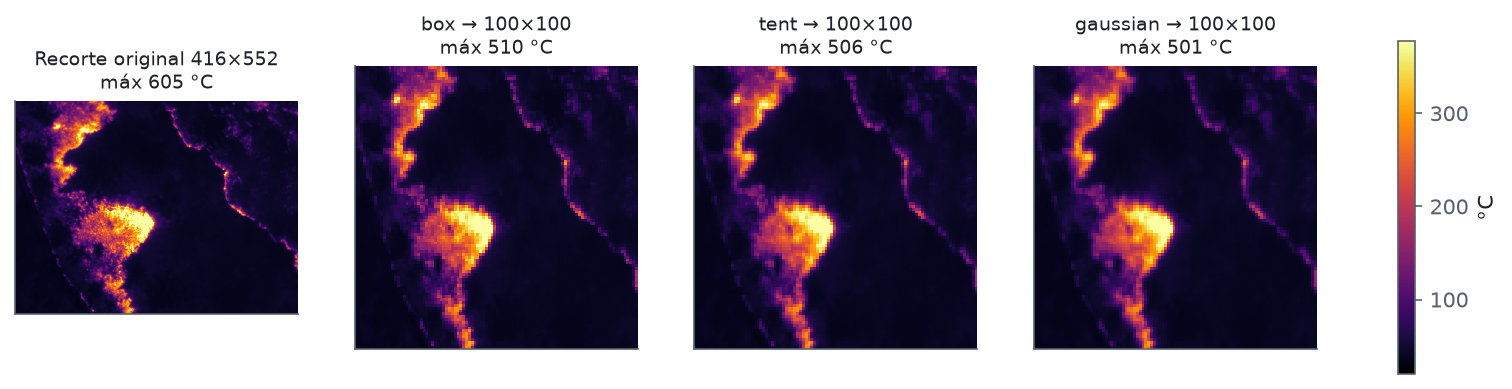
\includegraphics[width=\linewidth]{img/flame3_kernels.png}
	\caption{Comparación de kernels de reducción en la imagen con mayor temperatura de \textit{plot 1}.}
	\label{fig:flame3_kernels}
\end{figure}

\begin{figure}[H]
	\centering
	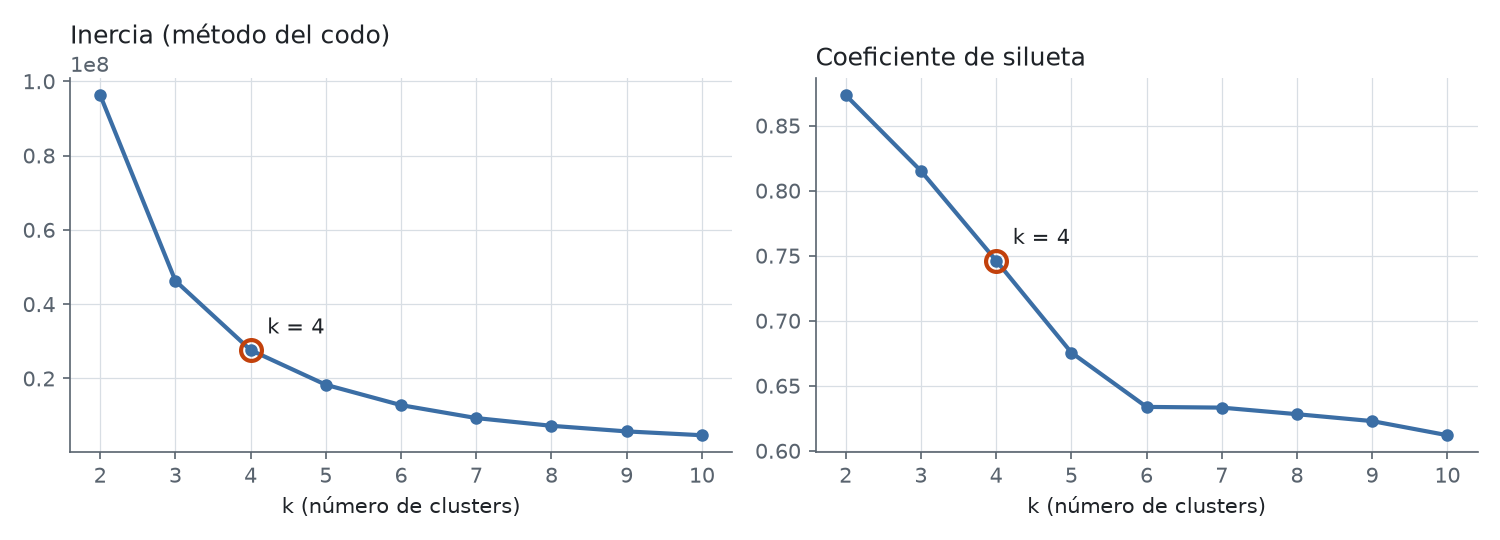
\includegraphics[width=0.9\linewidth]{img/flame3_k.png}
	\caption{Inercia y coeficiente de silueta de K-Means para $k = 2, \dots, 10$. El codo se encuentra en $k = 4$.}
	\label{fig:flame3_k}
\end{figure}

El resultado para \textit{plot 1} con $n = 100$ es una evolución de $296 \times 100 \times 100$ con cuatro estados (tabla \ref{tab:flame3_estados}). La proporción de estados evoluciona de forma suave: el frente cruza el encuadre, la quema alcanza su máximo alrededor de $t \approx 200$--$230$ y después la zona se enfría (figuras \ref{fig:flame3_frames} y \ref{fig:flame3_states}).

\begin{table}[H]
	\centering
	\begin{tabular}{c|c|c|c|l}
		\hline
		\textbf{Estado} & \textbf{Centroide} & \textbf{Rango} & \textbf{Fracción} & \textbf{Interpretación} \\ \hline
		0 & 35.8 °C & $< 56$ °C & 83.7\% & Suelo o vegetación sin quemar o ya fría \\ \hline
		1 & 76.1 °C & 56--116 °C & 11.4\% & Precalentamiento o rescoldo \\ \hline
		2 & 156.7 °C & 116--225 °C & 3.6\% & Combustión latente \\ \hline
		3 & 293.5 °C & $\geq 225$ °C & 1.3\% & Frente de llama \\ \hline
	\end{tabular}
	\caption{Estados obtenidos para \textit{plot 1} de FLAME 3.}
	\label{tab:flame3_estados}
\end{table}

\begin{figure}[H]
	\centering
	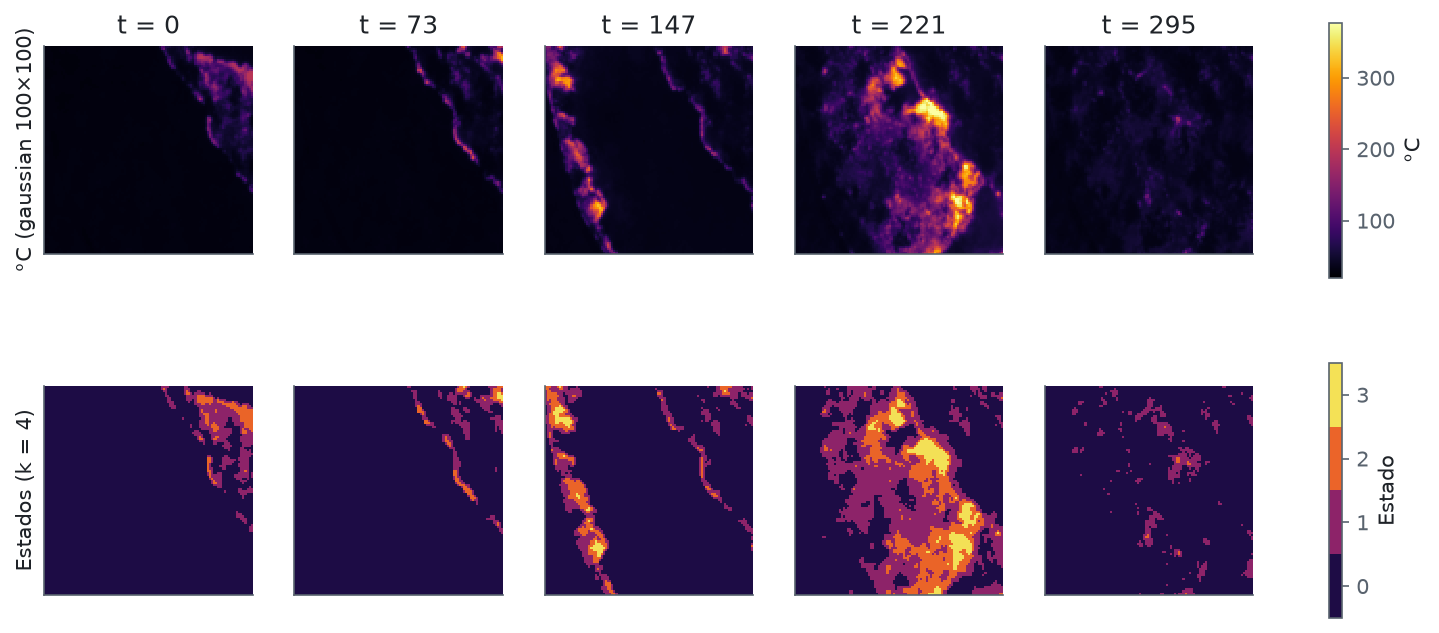
\includegraphics[width=\linewidth]{img/flame3_frames.png}
	\caption{Temperatura reducida a $100 \times 100$ y estados en cinco momentos de \textit{plot 1}.}
	\label{fig:flame3_frames}
\end{figure}

\begin{figure}[H]
	\centering
	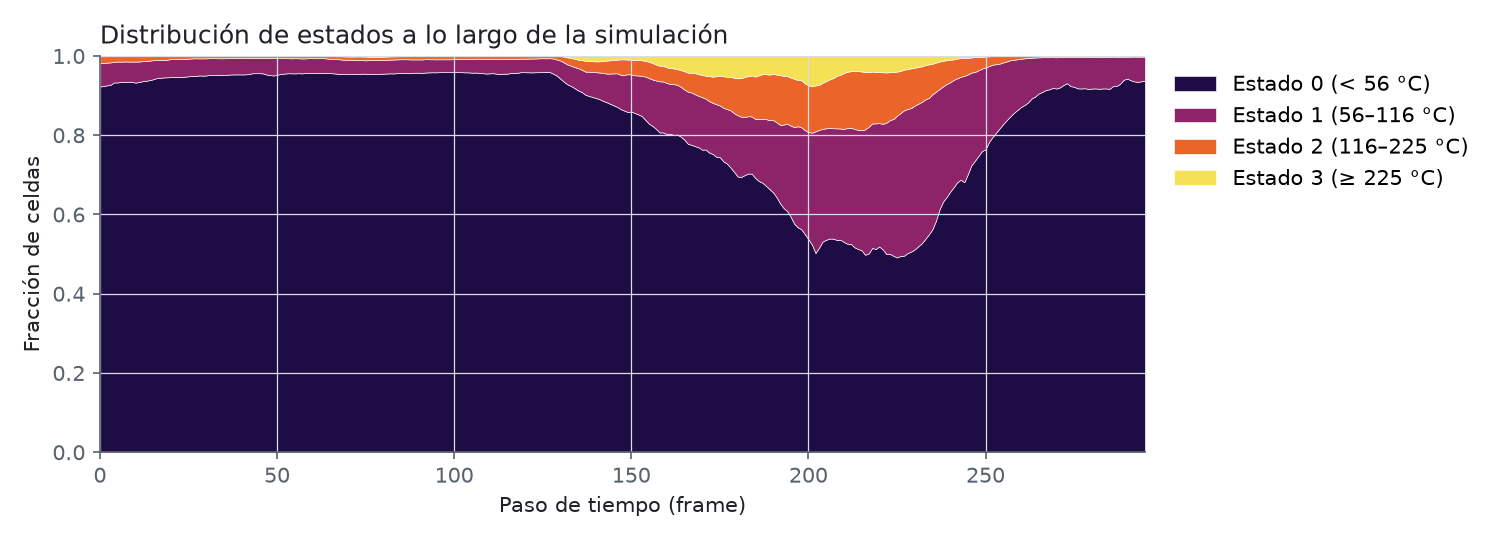
\includegraphics[width=0.9\linewidth]{img/flame3_states.png}
	\caption{Fracción de cada estado a lo largo de la secuencia de \textit{plot 1}.}
	\label{fig:flame3_states}
\end{figure}

\subsubsection{Entrenamiento y resultados}

\TODO{Entrenar el autómata celular neuronal con la evolución de \textit{plot 1} (4 estados, salida multiclase) y comparar la evolución generada contra la observada.}

\TODO{Procesar \textit{plot 2} (los GeoTIFF en °C aún no se descargan; solo se cuenta con los JPG) y evaluar si la regla aprendida en \textit{plot 1} generaliza.}
